\section{Introduction}
% Genaric Background Paragraph
A typical day in 2011 saw932,456 people cross into the U.S. (258,191 by air 48,073 by sea, and 621,874 by land) \cite{cpb_typical_2012}.
In addition there was 64,483 truck, rail and sea containers with 253,821 privately-owned vehicles \cite{cpb_typical_2012}.
As shown in Figure \ref{fig:PortalEntryMap} there are numerous entry points into the U.S. that are interconnected by a networks of rail and highways.
In the interadiciton of special nuclear mateiral it is desirable to detect and sieze the material before it enters into this complex network.
\begin{figure}
    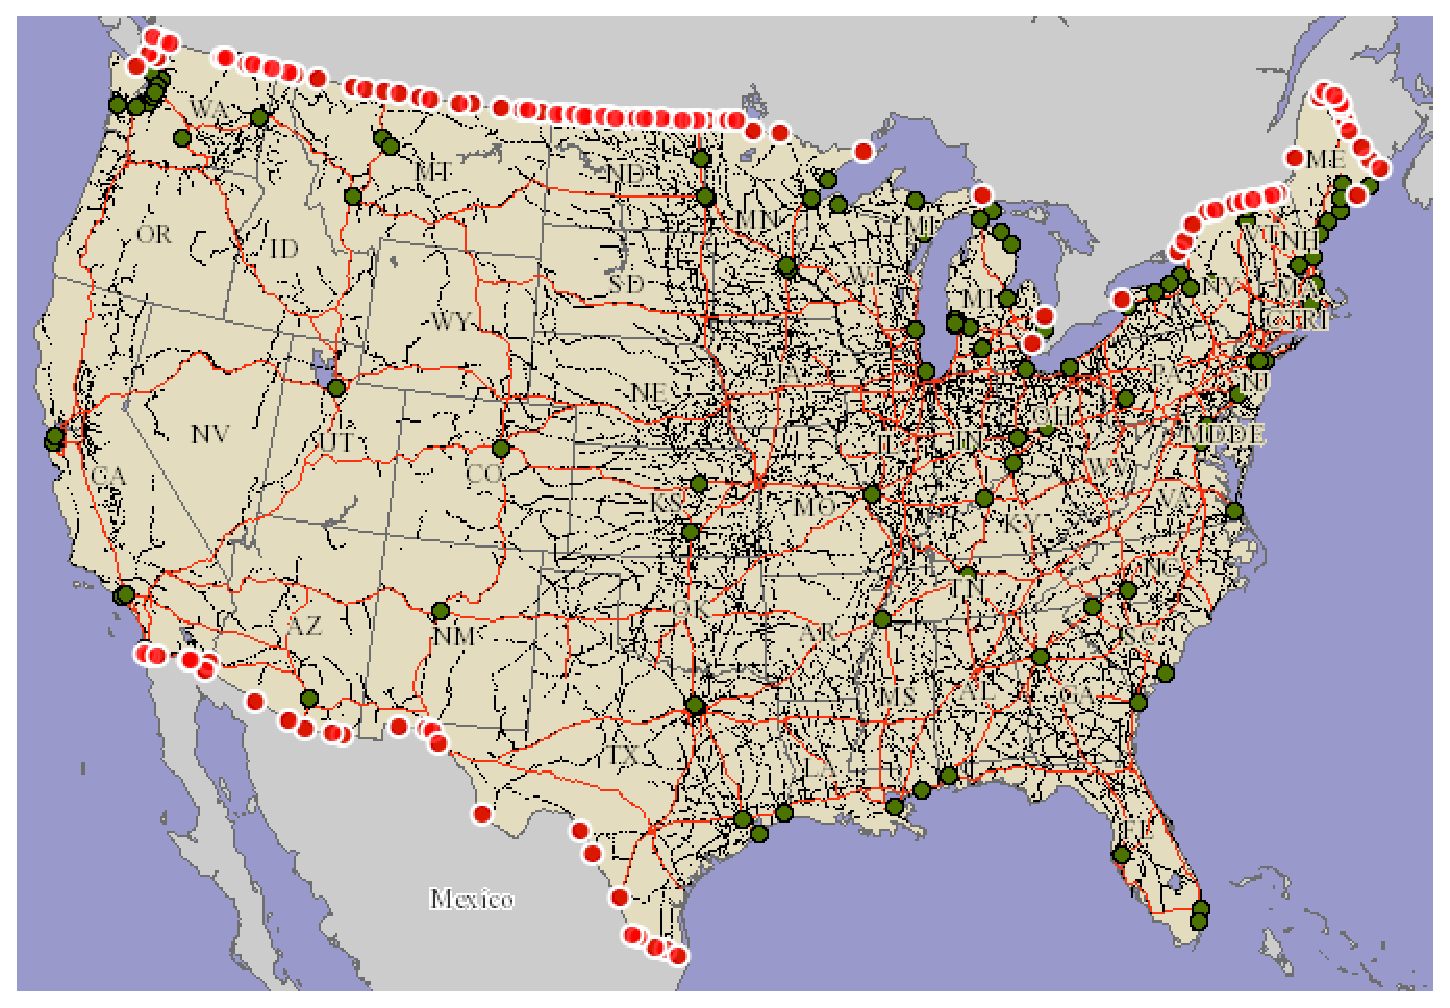
\includegraphics[width=\textwidth]{PortalEntryMap.eps}
    \label{fig:PortalEntryMap}
	\caption{Portal Entry Points into the U.S.}
\end{figure}
Radiation Portal Monitors (RPMs) are passive radiation detection systems implemented at over a thousand border corssings, designed to determine if cargo contains any nuclear material in a safe, nondestructive and effective manner\cite{kouzes_neutron_2010}.
The Department of Homeland Security (DHS) continues to fund research throught the Domestic Nuclear Detection Office (DNDO) in order to develop replacement technologies for the current \iso{He}{3} RPMs as \iso{He}{3} cannot be ecconomically replaced.
There are several alternatives to \iso{He}{3} being considered and all, with the exception of gas filled proportioinal detectors involve the dection of neutrons from scintillation events of the energy depsosited in the material from the neutron absorbtion reaction.
These detectors (among other requirements outline in Table \ref{tab:DHSCriteria}) must be able to efficienty discriminate between gamma (which can occur in medical isotopes) and neutrons (which are likely to be a signature of special nuclear material).
\begin{table}
	\centering
    \caption{Replacment Detector Requirements \protect\cite{kouzes_neutron_1999}}
	\begin{tabular}{c c }
	Parameter & Specification \\
	\hline
	\hline
	Absolute neutron detection efficiency & 2.5 cps/ng of ${}^{252}Cf$ (in specified test configuration) \\
	Intrinsic gamma-neutron detection efficiency & $ \epsilon_{int,\gamma n}\leq 10^{-6}$ \\
	Gamma absolute rejection ratio for neutrons (GARRn) & $ 0.9 \leq \text{ GARRn }\leq$ 1.1 at 10 mR/h exposure \\
	Cost &  \$ 30,000 per system \\
	\hline
	\end{tabular}
    \label{tab:DHSCriteria}
\end{table}

% Introduction to charged particles / energy deposition
Neutron detectors often utilize a material doped with an isotope of large thermal cross section for absorption such as \ios{Li}{6} or \iso{B}{10}. 
When these materials absorb a neutron the nucleus of the isotope becomes unstable and fisions into reaction products.
These reaction products (having an intial kinetic energy from the Q-value of the neutron absorbition reaction) travel through the material, transfering their kinetic energy to the material.
Photon interactions in the detector occur when a photon scatters of a single electron in a Compton scattering event (Table \ref{tab:ComptonScattering}).
\begin{table}
	\centering
    \caption{Maximum Energy of Secondary Electrons from Compton Scattering}
	\begin{tabular}{c | c c }
	& Photon Energy (MeV) & Maximum Compton Energy (MeV) \\
	\hline
	\hline
    \iso{Cs}{137} & 0.662 & 0.478 \\
    \iso{Co}{60} & 1.17, 1.33 & 0.960, 1160 \\
	\hline
	\end{tabular}
    \label{tab:ComptonScattering}
\end{table}
This Compton electron then produces a cascade of secondary electrons in the material, which depending upon the energy may or may not deposit a majority of it's energy in the detector.
The diffence in the transfer of kinetic energy from charged particle to electrons and from phton interactions (Compton scattering) to electrons introduces an oppertunity to exploit the differnece in energy deposition in order to maximize the discrimination between neutron and photon interactions in a detector.

